% =====================================================================
%  pu_class.tex -- the manual's figure of chapter 3 (Shock waves): the
%  class problem's first shock by impedance matching, drawn to scale.
%  In the style of the ME 697 Unit 6 sheet's pu_impact.tex (D. E.
%  Kittell). Built by 'make manual'.
%  The class deck's Hugoniots (input/me697_double_shock_2p00.deck):
%   Material X (right-facing, at rest): P = 1.60 (2.50 + 1.80 u - 0.04 u^2) u
%   Al flyer at 2.00 km/s (left-facing): P = 2.78 (5.30 + 1.34 w) w, w = 2 - u
%   (S2/C0 = -0.10/2.50 = -0.04 for Material X; S2 = 0 for Al.)
%  Solid: exact; dashed: acoustic, P = rho0 C0 u and rho0 C0 (2 - u).
%  Numbers (doc/manual/checks/ch3_shocks.py, 4a): exact u1 = 1.3713,
%  P1 = 10.736 GPa; acoustic u1 = 1.5730, P1 = 6.292 GPa.
% =====================================================================
\documentclass[tikz,border=10pt]{standalone}
\usepackage{amsmath}
\usetikzlibrary{arrows.meta}

\definecolor{slate}{HTML}{2C3E50}
\definecolor{oiblue}{HTML}{0072B2}
\definecolor{oiorange}{HTML}{E69F00}

\tikzset{
  axis/.style  = {-{Stealth[length=6pt]}, slate, thin},
  hugA/.style  = {oiblue, very thick},
  hugB/.style  = {oiorange, very thick},
  acA/.style   = {oiblue, thick, densely dashed},
  acB/.style   = {oiorange, thick, densely dashed},
  ext/.style   = {slate, thin, densely dotted},
  state/.style = {font=\small, text=slate},
}

\begin{document}
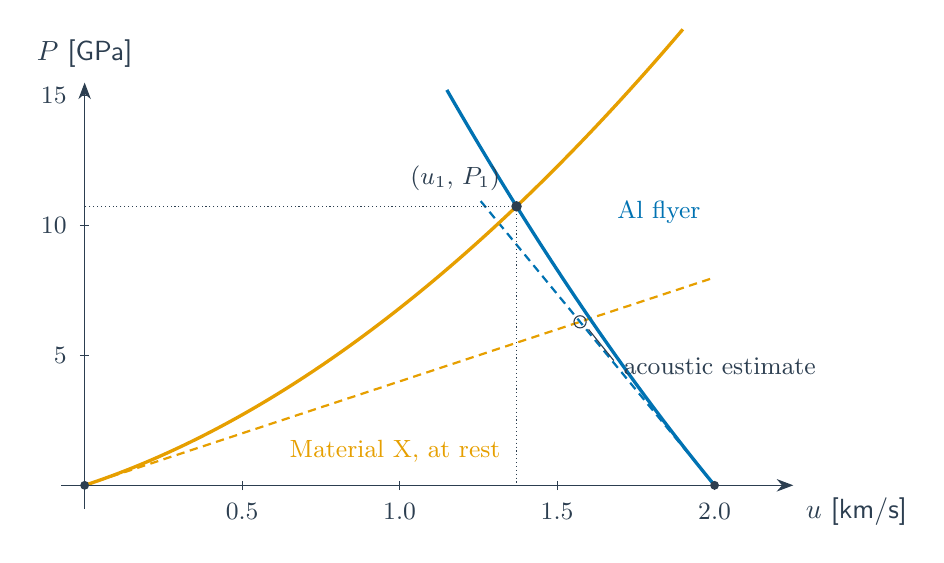
\begin{tikzpicture}[font=\sffamily, text=slate,
    declare function={
      U(\u)  = \u*4.0;      % cm per km/s
      Yp(\p) = \p*0.33;     % cm per GPa
      PB(\u) = 1.60*(2.50 + 1.80*\u - 0.04*\u*\u)*\u;
      PA(\u) = 2.78*(5.30 + 1.34*(2-\u))*(2-\u);
    }]

  % ---- acoustic (dashed, approximate) ----
  \draw[acB] (0,0) -- ({U(2.0)}, {Yp(8.0)});
  \draw[acA] ({U(2.0)}, 0) -- ({U(1.25)}, {Yp(14.73*0.75)});

  % ---- exact Hugoniots (solid) ----
  \draw[hugB] plot[domain=0:1.9, samples=120] ({U(\x)},{Yp(PB(\x))});
  \draw[hugA] plot[domain=1.15:2.0, samples=120] ({U(\x)},{Yp(PA(\x))});

  % ---- states ----
  \draw[ext] ({U(1.3713)}, {Yp(10.736)}) -- ({U(1.3713)}, 0);
  \draw[ext] ({U(1.3713)}, {Yp(10.736)}) -- (0, {Yp(10.736)});
  \fill[slate] (0, 0) circle (1.6pt);
  \fill[slate] ({U(2.0)}, 0) circle (1.6pt);
  \fill[slate] ({U(1.3713)}, {Yp(10.736)}) circle (1.9pt);
  \node[state, anchor=south east] at ({U(1.35)}, {Yp(10.95)})
      {$\left(u_1,\,P_1\right)$};
  \draw[slate] ({U(1.5730)}, {Yp(6.292)}) circle (2.2pt);
  \node[state, anchor=west] at ({U(1.68)}, {Yp(4.6)})
      {acoustic estimate};
  \draw[slate, thin] ({U(1.60)}, {Yp(6.0)}) -- ({U(1.68)}, {Yp(4.8)});

  % ---- curve labels ----
  \node[state, text=oiorange, anchor=west] at ({U(0.62)}, {Yp(1.3)})
      {Material X, at rest};
  \node[state, text=oiblue, anchor=west] at ({U(1.66)}, {Yp(10.5)})
      {Al flyer};

  % ---- axes ----
  \draw[axis] (-0.3, 0) -- ({U(2.25)}, 0) node[below right=1pt] {$u$ [km/s]};
  \draw[axis] (0, -0.3) -- (0, {Yp(15.5)}) node[above=2pt] {$P$ [GPa]};
  \foreach \u/\l in {0.5/0.5, 1.0/1.0, 1.5/1.5, 2.0/2.0} {
    \draw[slate, thin] ({U(\u)}, -0.06) -- ({U(\u)}, 0.06);
    \node[below=3pt, font=\small] at ({U(\u)}, 0) {\l};
  }
  \foreach \p in {5, 10, 15} {
    \draw[slate, thin] (-0.06, {Yp(\p)}) -- (0.06, {Yp(\p)});
    \node[left=3pt, font=\small] at (0, {Yp(\p)}) {\p};
  }
\end{tikzpicture}
\end{document}
